\chapter{Complex Spaces}


It is time to embrace complex numbers. A complex vector space is one where all of the numbers that we previously assumed were real can now be complex: $\RR \to \CC$. This means that a linear combination of vectors $\alpha\vec{v}+ \beta\vec{w}$ may have complex coefficients, $\alpha,\beta\in\CC$. 

\section{Review of complex numbers}

A complex number has a real and imaginary part. The imaginary part is proportional to  $i \defeq \sqrt{-1}$. We typically write complex numbers $z$ in either the Cartesian or polar form:
\begin{align}
    z &= x+iy 
    &
    z &= r \e^{i\theta}
    \ .
\end{align}
Here $x,y,r$, and $\theta$ are real parameters. The radius is greater than zero ($r>0$) and the angle $\theta$ is defined modulo $2\pi$ so that $\e^{i(\theta+2\pi)} = \e^{i\theta}$.

\paragraph{Are complex numbers a vector space?}
In the Cartesian expression, you might be tempted to read this like a vector space with two basis vectors: $\ket{e_1}=1$ and $\ket{e_2} = 2$ and a complex number $z$ is the linear combination of basis vectors $\ket{z} = x \ket{e_1} + y \ket{e_2}$. The addition rule for complex numbers reaffirms this:
\begin{align}
    (a+ib)+ (x+iy) = (a+x) + i (b+y) \ .
\end{align}
So we can see that complex numbers have the same structure as the vector space $\RR^2$. However, it is incorrect to think that the vector space $\RR^2$ is the same as complex numbers, $\CC$. This is because complex numbers have additional structure beyond that of a vector space---in fact, beyond even that of a metric space. 

This additional structure is a rule by which two `vectors' can be multiplied to produce another vector. We have no such rule in a general vector space.\sidenote{And don't even get me started on the cross product. That is only valid in three dimensions due to a coincidence in the dimensionality of the Hodge dual of two vectors, see Section~\ref{sec:cross:product}.} The rule $i^2 = -1$ means that
\begin{align}
    (a+ib)(x+iy) = (ax - by) + i (ax + by) \ .
\end{align}
Thus complex numbers are a vector space \emph{with additional structure}. The nature of this additional structure is outside the scope of this course, but you can learn more about it in a field called \textbf{geometric algebra}.\footnote{One of my favorite overviews of this field is Jack Rusher's talk ``From Geometry to Algebra and Back Again: 4000 Years of Papers'' at the Strange Loop Conference, \url{https://youtu.be/1cRFfYQYGxE?si=x9U0mIfeqXy3QHLd}. Another nice one is YouTuber sudgylacmoe's ``Swift Introduction to Geometric Algebra,'' \url{https://youtu.be/60z_hpEAtD8}.}\autocite{Doran:2007tqa} This topic has some really neat manifestations in rotational dynamics\footnote{\url{https://www.youtube.com/watch?v=BN4coAyF5PE&feature=youtu.be}}\autocite{10.1119/5.0109883}, relativity\autocite{10.1119/1.4734014}, and electrodynamics\footnote{\url{https://youtu.be/WN_4j8v6cXo}}\autocite{Dressel:2014fna}.

\paragraph{The exponential}
The polar form of a complex number is related to the Cartesian form through Euler's identity:
\begin{align}
    \e^{i\theta} = \cos\theta + i\sin\theta
\end{align}
This identification is somewhat mysterious the first time you see it.\sidenote{Perhaps it remains mysterious and most of us simply get used to it.} One way to appreciate this is to connect it to the definition of the exponential as a repetition of many small transformations:
\begin{align}
    \e^x \defeq \lim_{n\to\infty} 
    \prod _n \left(1+\frac{x}{n}\right)^n \ .
\end{align}
The right-hand side is a product of factors $(1+\epsilon)$ where $\epsilon = x/n$ is a \emph{small} shift in the $x$ direction.\sidenote{For real numbers, there is only one direction: the real axis. But there are often cases where $x$ is a more sophisticated object, such as a matrix.} As $n\to\infty$, the factor $(1+\epsilon)$ is thus a small transformation and the exponential is the product of $n\to\infty$ of these small transformations. 

\begin{example}[Exponential representation of rotations.] Consider rotations in two dimensions. An infinitesimal rotation is:
\begin{align}
    R(1+\epsilon) = 
    \begin{pmatrix}
        1 & -\varepsilon \\
        \varepsilon & \pp 1
    \end{pmatrix}
    = 
    \one + \varepsilon 
    \begin{pmatrix}
        0 & - 1 \\
        1 & \pp 0
    \end{pmatrix} \ .
\end{align}
You can check that this is exactly what you get from a first-order Taylor expansion of the rotation matrix:
\begin{align}
    R(\theta) = 
    R(0)
    + \theta 
    \frac{\D{}}{\D{\theta}}  + \mathcal O(\theta^2) \ .
\end{align}
Please explicitly write out the two matrices on the right-hand side if this is not clear. 

The matrix 
\begin{align}
    T =\begin{pmatrix}
        0 & - 1 \\
        1 & \pp 0
    \end{pmatrix} 
\end{align}
has a special name: it is the \textbf{generator} of rotations. We may write a finite rotation matrix as the exponentiation of this generator:
\begin{align}
    R(\theta)  = 
    \lim_{n\to\infty} \frac{1}{n}
    \left(1+\frac{\theta}{n} T\right)^n
    = 
    \e^{i\theta T} \ .
\end{align}
You may also explicitly write out the first few terms of $e^{i\theta T}$ as a power series to see that the even terms show up on the diagonal and the odd terms show up on the off-diagonal. The terms sum to the usual cosine and sine expansions.
\end{example}

The imaginary number $i$ acts as a rotation in the complex plane.\sidenote{This is `obvious' when writing $i=\e^{i\pi/2}$, but here we are motivating the exponential representation and so cannot use the exponential representation to motivate itself.} Taking a complex number $z$ and multiplying it by $(1+i\epsilon )$ returns a complex number $z'$ that is approximately $z$ but rotated by a small angle $\epsilon$. The length of $z'$ is the same as the length of $z$ up to factors of $\mathcal O(\epsilon^2)$.
\begin{exercise}
The length of a complex number $z=a+ib$ is $|z| = \sqrt{a^2 + b^2}$. Show that the lengths of $z$ and $(1+i \epsilon )z$ have the same length up to corrections of order $\mathcal O(\epsilon^2)$.
\end{exercise}
Thus the polar form $z=r\e^{i\theta}$ is (1) rescaling by a real number $r$, and (2) a rotation by an angle $\theta$ in the complex plane. 


\section{Phasors}

This section is outside the main scope of this course.

One way that both the Cartesian and the polar pictures of a complex number come together is something called a \textbf{phasor diagram}\index{phasor}, shown in Figure~\ref{fig:figure:phasor}.
\begin{marginfigure}%[th]
    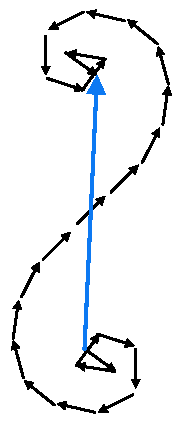
\includegraphics[width=.5\textwidth]{figures/Phasor.pdf}
    \captionsetup{font={scriptsize,sf}}
    \caption{Example of a phasor diagram showing the sum, in blue, of many complex numbers of unit length. Each complex number is $\hat z = e^{iS[q]}$, where $q$ represents a path. The function $S$ is an action. The middle of the diagram is the region where the action is minimized so that it does not change appreciably over nearby paths. This region of \emph{least action} dominates in the classical limit, where the spirals become tighter.}
    \label{fig:figure:phasor}
\end{marginfigure}
At its heart, a phasor is simply a complex number of unit length. That means it is of the form $\hat z = e^{i\theta}$. 
Phasors are a nice way to think about an object at the heart of quantum mechanics: the path integral. I strongly recommend reading Feynman's popular science book, \emph{QED: The Strange Theory of Light and Matter}\autocite{Feynman:1986er}. The material is based on Feynman's Douglas Robb memorial lectures.\sidenote{You may still be able to find recordings of these lectures online.}
% 
Richard Feynman developed the path integral formulation of quantum mechanics in his Ph.D thesis\autocite{Feynman:1942us}. The proposal is that the probability amplitude\sidenote{The probability amplitude $\psi$ is a complex number whose magnitude squared $|\psi|^2 = \psi^*\psi$ is the probability.} to go from state $A$ to state $B$ is given by a sum of phasors up to a normalization\sidenote{The perceptive reader will note that this is an important point that I'm ignoring. This normalization assures that there are no probabilities greater than one.} that we do not belabor here. Each phasor represents the probability amplitude for a particular path between $A$ and $B$. 
\begin{example}
Consider the double slit experiment. There are two paths, one from either slit. Each path is associated with a complex number of unit modulus. The probability amplitude is the sum of the phasors for each path. 
\end{example}
The probability amplitude is thus
\begin{align}
    \Psi(A\to B) \propto \sum_\textnormal{path}
    \e^{iS[q_\textnormal{path}]/\hbar} \ ,
\end{align}
where $q_\textnormal{path}(t)$ is some trajectory that goes from $A$ to $B$ as a function of time $t$. The function $S[q]$ is the usual action that you met in mechanics: it is the time integral over the Lagrangian, $S=\int\D{t}\, L[q]$, which is itself the difference between kinetic and potential energy. The number $\hbar$ is Planck's constant; it is required by dimensional analysis and with respect to human scales it is quite small.

Figure~\ref{fig:figure:phasor} shows that when the action changes quickly as a function of $q$, the phase in $e^{iS[q]}$ changes quickly and the amplitude contribution from nearby paths cancel each other out. However, the paths near the minimum of the action $S'[q]=0$ have a nearly constant action and so those phasors add constructively. The contribution to the amplitude is dominated by these paths that minimize the action. The classical limit of quantum mechanics is the case where $\hbar \to 0$ so that the action varies so rapidly that only the path of minimal action contributes. This is the quantum mechanical `derivation' of the so-called \emph{principle of least action}.

Phasors are not used much in modern physics, but the intuition of the phasor picture of the path integral is at the heart of quantum field theory. By a curious relation between quantum and statistical physics, this is closely related to statistical field theory by a factor of $i$.



\section{Complex vector space}

A complex vector space is one where all `numbers' are now understood to be \emph{complex numbers}. This means that the components of vectors, matrices, and all tensors are complex. It means that you may take linear combinations of objects with complex coefficients. 

Observe that because complex numbers basically have the same arithmetic as real numbers---up to this funny $i^2=-1$ business---nothing really changes from the \emph{vector space} perspective. We still write vectors as
\begin{align}
    \ket{v} = v^i\ket{e_i}
\end{align}
with the understanding that $v^i$ is now a number of the form $v^i = a^i + i b^i$.\sidenote{Please do not confused the index $i$ with the imaginary number $i$. Some people use Greek letter iota $\iota$ instead of $i$, but I find that this looks like a typo where someone lost the dot.}
\begin{example}
Suppose you are in a three-dimensional  complex vector space with a vector $\ket{v}$ whose components are
\begin{align}
    v^1 &= 2+i
    &
    v^2 &= 3i
    &
    v^3 &= -2 \ .
\end{align}
Suppose you have a dual vector $\bra{w}$ whose components are
\begin{align}
    w_1 &= -i
    &
    w_2 &= 1+i
    &
    w_3 &= 2 \ .
\end{align}
Then the action of $\bra{w}$ on $\ket{v}$ is
\begin{align}
    \la w \mid v \ra &=
    (2+i)(-i)+(3i)(1+i)+(-2)2 
    =
    -7 + i
    \ . 
\end{align}
\end{example}


In the above example, observe that we never invoked a metric. Everything so far has been for a complex \emph{vector space} with no mention of the existence of a metric. 

Secondly, note that we have nothing to say about basis vectors, $\ket{e_i}$. Of course we still have basis vectors, $\ket{e_i}$, and an accompanying basis of dual vectors $\bra{e^i}$. But there is nothing different about them. We do not even have to `complexify' them! One of the big deals of linear algebra has been that we can completely abstract away what the basis vectors \emph{mean}. Whether the vector space is real or complex is purely a statement about the \emph{coefficients}---the \emph{numbers}. The abstract `vector-ness' or `tensor-ness' of different types of objects remain as abstract as before.\sidenote{To remind you: there is a basis of vectors that encodes some abstraction. It may encode velocities, differential operators, functions defined on the sphere, Fibonacci sequences, etc. Then we define linear maps on these abstract objects: this gives us dual vectors, matrices, and all other form of tensor.}



\section{Inner product on complex spaces}

Things become a bit more interesting when we complexify a metric space. We have to update our rules a bit. Previously we assumed that the metric is symmetric, $\langle v, w\rangle = \langle w, v\rangle$. This turns out to only be true for real spaces. When we have a complex vector space, the metric must satisfy symmetry with a complex conjugation:
\begin{align}
    \la v, w \ra = \la w, v \ra^* \ .
    \label{eq:complex:metric:star}
\end{align}
That is a little unusual. The general inner product is \emph{not} symmetric!

\subsection{Anti-Linearity}

One way of expressing \eqref{eq:complex:metric:star} is to say that the inner product is \textbf{antilinear}\index{antilinear} in its first component while it is linear in the second component. The word `antilinear' means that somewhere there is a complex conjugation.\sidenote{The most famous anti-linear operation in physics is time reversal. This is not something we can do in an experiment, but theoretically we can flip the direction of time in all of our equations.} This means that for complex numbers $a$ and $b$,
\begin{align}
    \la av + bu, w \ra = 
    a^* \la v, w\ra
    +
    b^* \la v, w\ra
\end{align}
whereas 
\begin{align}
    \la v, aw + bu \ra = 
    a \la v, w\ra
    +
    b \la v, u\ra \ .
\end{align}


\subsection{Norms are Real}
The norm of a complex vector is real. 
\begin{align}
    |v|^2 = \la v, v \ra = \la v, v \ra^* \ .
\end{align}
In my opinion this helps justify the notation $|v|$ for the magnitude of a vector.\sidenote{What really annoys me is that sometimes we write $|M|$ to mean the determinant of a matrix. This almost makes sense because the determinant is some intrinsic number associated with a matrix. However, the determinant can be positive or negative. This gets confusing when one needs to take the absolute value of a determinant and you do not know if $|M|$ means $\det M$ or $|\det M|$.}


\subsection{Metric}
In real space we defined the metric as the symmetric (0,2) tensor that encodes the linear transformation $V\times V \to \mathbbm{R}$ that is the inner product:
\begin{align}
    \la v , w \ra = g_{ij}v^i w^j 
    &
    g_{ij} = g_{ji}
    \ .
\end{align}
In complex space we sometimes\sidenote{You can opt not to do this. In fact, one does not often have an occasion to write out a complex space metric explicitly for most undergraduate physics courses.} write the metric with funny indices $\bar{\imath}$ and $\bar{\jmath}$ instead of $i$ and $j$ to differentiate the first and second components of $g_{\bar{\imath}j}$. This is necessary now that the inner product is no longer symmetric, but is rather symmetric up to a complex conjugation. We write:
\begin{align}
    \la v, w \ra &= g_{\bar{\imath}j}(v^*)^{\bar{\imath}}w^j \ .
\end{align}
Here $(v^*)^{\bar{\imath}}$ is simply $(v^i)^*$.

The inner product rule \eqref{eq:complex:metric:star} then tells us that
\begin{align}
    g_{\bar{\imath}j}(v^*)^{\bar{\imath}}w^j \ .
    &= 
    \left(
        g_{\bar{\jmath}i}
        (w^*)^{\bar{\jmath}}
        v^i
        \right)^*
    \\
    &= 
    g_{j\bar{\imath}}^* w^j(v^*)^{\bar{\imath}}
     \ .
\end{align}
From this we find that the metric satisfies
\begin{align}
g_{j\bar{\imath}}^* =
    g_{\bar{\imath}j} \ ,
\end{align}
where we write $g_{j\bar{\imath}}^* = (g_{\bar\imath j})^*$.  This result is not particularly surprising: the metric has the same symmetry property as the inner product. 


\subsection{Adjoint}

% What about the adjoint of a transformation? For a real vector space, the adjoint is simply the transpose. For a complex vector space, the adjoint is the transpose \emph{and} a complex conjugation on each component.
% :
% \begin{align}
%     (A^\dag)\aij{i}{j} = g^{ik}(A\aij{\ell}{k})^*g_{\ell j} \ .
% \end{align}

Recall that the adjoint of a matrix $A$ is defined by
\begin{align}
    \la A v , w \ra \defeq 
    \la v, A^\dag w \ra \ .
\end{align}
We would like to relate the components of $A^\dag$ to $A$ in a complex space. The components of $A$ in a basis $\ket{e_i}$ are 
\begin{align}
    A\aij{i}{j} = \la e^i \mid A \mid e_j \ra 
    = \la e_i, A e_j \ra \ .
\end{align}
Using \eqref{eq:complex:metric:star} we may then write:
\begin{align}
    (A^\dag)\aij{i}{j}
    = 
    \la e_i, A^\dag e_j \ra
    =
    \la A e_i, e_j \ra
    =
    \la e_j, A e_i \ra^*
    =
    (A\aij{j}{i})^* \ .
\end{align}
This means, for example, in matrix form:
\begin{align}
    \begin{pmatrix}
        A\aij 11 & A\aij 12 \\
        A\aij 21 & A\aij 22 
    \end{pmatrix}^\dag &= 
    \begin{pmatrix}
        (A\aij 11)^* & (A\aij 21)^* \\
        (A\aij 12)^* & (A\aij 12 )^*
    \end{pmatrix} \ .
\end{align}
In a complex space, the adjoint of a matrix is a combination of the transpose and the complex conjugate. This is sometimes called the \textbf{Hermitian conjugate}\index{Hermitian conjugate}.\sidenote{The Hermitian conjugate and the adjoint or a matrix are the same.} For real vector spaces, the adjoint reduces to the transpose. 


\begin{example}
Here's the adjoint of an explicit matrix:
\begin{align}
\begin{pmatrix}
        3.5 +2i & 2.3+7i \\
        8.3 + 5i & 5-2i
    \end{pmatrix}^\dag &= 
    \begin{pmatrix}
        3.5 -2i &  8.3 - 5i\\
        2.3 -7i & 5 +2i
    \end{pmatrix} \ .
\end{align}
\end{example}

It is also useful to consider the adjoint of a product of matrices, $AB$. We can see that
\begin{align}
    \la AB \vec{v}, \vec{w} \ra
    =
    \la B \vec{v},  A^\dag \vec{w} \ra
    =
    \la \vec{v}, B^\dag A^\dag \vec{w} \ra \ .
\end{align}
This tells us that
\begin{align}
    (AB)^\dag = B^\dag A^\dag \ .
    \label{eq:adjoint:of:product}
\end{align}



\begin{example} What do isometries look like in a complex vector space? Let us suppose that we have the Euclidean metric (even though the space is now complex):
\begin{align}
    g_{\bar\imath j} = \text{diag}(1,1,\cdots, 1) = \mathbbm{1} \ .
\end{align}
Let $U$ be an isometry in this space; this is a conventional name whose meaning will be clear soon. The condition for an isometry in this space is that a transformation $\ket v \to U\ket{v}$ preserves the metric. Observe that because the metric is not symmetric, but rather symmetric-up-to-a-conjugate, it is useful to write the inner product using brackets rather than simply index contraction. We have:
\begin{align}
    \la U\vec{v}, U\vec{w} \ra = \la \vec{v}, U^\dag U \vec{w} \ra \stackrel{?}{=} \la \vec{v}, \vec{w} \ra \ .
\end{align}
This tells us that the condition for $U$ to be an isometry is that $U^\dag U = \mathbbm{1}$. Matrices that satisfy this are called \textbf{unitary} matrices, thus justifying the name $U$. 
\end{example}

\begin{example}
The usual rotation matrices (obviously!) satisfy the unitary condition. Thus rotations are a simple example of a unitary matrix. There are more complicated unitary matrices, for example in two complex dimensions:
\begin{align}
    U(\theta) = 
    \begin{pmatrix}
        e^{i\theta} & 0\\
        0 & e^{-i\theta}
    \end{pmatrix}
    \label{eg:unitary:matrix:diagonal}
\end{align}
is a transformation that rephases the first $v^1 \to e^{i\theta}v^1$  and second $v^2 \to e^{-i\theta}v^2$ components of a vector by opposite phases. It should be obvious that $U^\dag U = \one$. 
\end{example}


\begin{exercise}
A bonus observation: show that \eqref{eg:unitary:matrix:diagonal} can be understood as a Taylor expansion with respect to a matrix $T$:
\begin{align}
    U(\theta) &= \sum_{n=0}^\infty \frac{\theta^n}{n!} (iT)^n
    &
    iT=
    \begin{pmatrix}
        i & 0\\
        0 & -i
    \end{pmatrix} \ .
\end{align}
The matrix $T$ is called the \textbf{generator} of the isometry $U$. 
\end{exercise}


\begin{exercise}
Show that the generator of rotations is
\begin{align}
    R(\theta) &= \sum_{n=0}^\infty \frac{\theta^n}{n!} (iT)^n
    &
    iT=
    \begin{pmatrix}
        0 & -1\\
        1 & \pp 0
    \end{pmatrix} \ .
\end{align}
The curious choice of defining $iT$ is so that the generator $T$ is Hermitian, $T^\dag = T$, which is a common convention in physics.
\end{exercise}


% \begin{table}
%     \renewcommand{\arraystretch}{1.3} % spacing between rows
%     \centering
%     \begin{tabular}{ @{} llllll @{} } \toprule % @{} removes space
%         Space
%         & Numbers
%         & Inner Product
%         & Contraction
%         & Matrix
%         & Identity
%         \\ \hline
%         Classic
%             & vector
%             & row-vector
%             & 
%             &       
%         \\
%             & $\vec{v} = v^i \bas{e}_i$
%             & $\row{w} = w_i \rbas{e}^i$
%             & $\rbas{e}^i\bas{e}_j = \delta^i_j$
%             & $M=M\aij{i}{j} \bas{e}_i\otimes \rbas{e}^j$
%             & $\one$
%         \\ \hline
%         Quantum 
%             & ket
%             & bra
%             &       
%             &
%         \\
%             & $\ket{v} = v^i\ket{i}$
%             & $\bra{w} = w_i \bra{i}$
%             & $\langle i | j\rangle = \delta^i_j$
%             & $M=M\aij{i}{j} \ket{i}\bra{j}$
%             & $\ket{i}\bra{i}$
%         \\ \bottomrule
%     \end{tabular}
%     \caption{
%         Dictionary between `classic' notation and `quantum' (bra--ket) notation.
%         \label{tab:classic:bra:ket:dictionary}
%     }
% \end{table}

\section{Self-Adjoint Matrices}

\textbf{Self-adjoint matrices} are those for which
\begin{align}
M^\dag = M \ .     
\label{eq:self:adjoint}
\end{align}
These are known equivalently as \textbf{Hermitian matrices}\index{Hermitian matrix}.
These are what we mean by `nice' matrices. They generalize the notion of symmetric matrices. 
\begin{example}
The \textbf{Pauli matrices} are a set of three $2\times 2$ Hermitian matrices:
\begin{align}
    \sigma^1
    &=
    \begin{pmatrix}
        0 & 1 \\
        1 & 0
    \end{pmatrix}
    &
    \sigma^2
    &=
    \begin{pmatrix}
        0 & -i \\
        i & \pp 0
    \end{pmatrix}
    &
    \sigma^3
    &=
    \begin{pmatrix}
        1 & \pp 0 \\
        0 & -1
    \end{pmatrix} \ .
\end{align}
\end{example}
\begin{exercise}
Show that any \emph{real} linear combination of the Pauli matrices is a Hermitian matrix:
\begin{align}
    a \sigma^1 + b \sigma^2 + c\sigma^3 \ .
\end{align}
Here the numbers $a$, $b$, and $c$ are real. Explain what goes wrong if these numbers are complex---in that case the matrix is no longer Hermitian.

Argue that \emph{all} $2\times 2$ Hermitian matrices take the above form. Yes, this means that the Pauli matrices are a basis for the space of $2\times 2$ Hermitian matrices, which is itself a \emph{real} vector space because the coefficients $a$, $b$, and $c$ are real.
\end{exercise}

% \subsection{Eigen-bra}

% If $\ket{\xi}$ is a normalized eigenvector of the matrix $M$ with eigenvalues $\lambda$, $M\ket{\xi} = \lambda\ket{\xi}$, then 
% \begin{align}
%     \la v, M \xi \ra = \lambda \la v, \xi \ra 
%     \ .
% \end{align}
% Similarly, if we use the definition of the adjoint:
% \begin{align}
%     \la v, M \xi \ra = \la M^\dag\xi, v \ra 
%     = \bar\lambda^* \la \xi, v \ra
%     = \bar\lambda^* \la v, \xi \ra^*
%     \ .
% \end{align}
% Here $\bar\lambda$ is the eigenvalue of $M^\dag$ on $\ket{\xi}$. We have used the antilinearity of the inner product with respect to its first component. 




\subsection{Eigenvalues}

Here is the first really neat thing about nice matrices:
\begin{theorem}[Real eigenvalues]
The eigenvalues of self-adjoint matrices are real.
\end{theorem}
\begin{proof}
Let $M=M^\dag$ be a self-adjoint matrix. Let $\ket{\xi}$ be  an eigenvector eigenvalue $\lambda$:
\begin{align}
    M\ket{\xi} &= \lambda\ket{\xi} 
    \ .
\end{align}
Then consider:
\begin{align}
    \la M \xi, \xi \ra 
    = 
    \la \lambda \xi, \xi \ra
    = 
    \lambda^* \la \xi, \xi \ra \ .
\end{align}
Using the adjoint, we may also write this as
\begin{align}
    \la M \xi, \xi \ra 
    = 
    \la \xi, M^\dag \xi \ra
    =
    \la \xi, M \xi \ra
    = 
    \lambda \la \xi, \xi \ra \ .
\end{align}
Taking the difference of these two expressions gives
\begin{align}
    \left(\lambda^*-\lambda\right) \la \xi, \xi \ra  = 0 \ .
\end{align}
We know that $ \la \xi, \xi \ra\neq 0$, which means that $\lambda^* = \lambda$. This means that $\lambda$ is pure real. 
\end{proof}
Because real vector spaces are complex vector spaces with  a restriction to real coefficients, this theorem holsd for real vector spaces as well. 

\subsection{Eigenvectors}

Here is the second really neat thing about nice matrices:
\begin{theorem}[Orthogonal eigenvectors]
The eigenvectors of self-adjoint matrices are orthogonal.
\end{theorem}
\begin{proof}
Let $M=M^\dag$ be a self-adjoint matrix. Let $\xi_a$ and $\xi_b$ be two distinct eigenvectors ($b\neq a$) with distinct eigenvalues $\lambda_a \neq \lambda_b$:
\begin{align}
    M\ket{\xi_a} &= \lambda_a\ket{\xi_a} 
    &
    M\ket{\xi_b} &= \lambda_b\ket{\xi_b} 
    \ .
\end{align}
Then we may consider
\begin{align}
    \la M \xi_a, \xi_b \ra 
    &= 
    \la \xi_a, M^\dag \xi_b \ra 
    =
    \la \xi_a, M \xi_b \ra
    .
\end{align}
We may use $\la M \xi_a, \xi_b \ra = \la \xi_b, M \xi_a \ra^* = \lambda_b^*\la \xi_a, \xi_b \ra$ to then write
\begin{align}
    (\lambda_a - \lambda_b)\la \xi_a,\xi_b\ra = 0 \ .
\end{align}
We have used $\lambda_a^* = \lambda^a$ since $M$ is self-adjoint. Because $\lambda_a\neq \lambda_b$, we must have that $\la \xi_a, \xi_b\ra = 0$. This means that the two eigenvectors are orthogonal. 
\end{proof}
Given a set of orthogonal eigenvectors, one may normalize them by dividing by their lengths to produce an orthonormal eigenbasis. 

\subsection{Physical observables and nice bases}

What is the significance of all this? 

\paragraph{Real eigenvalues}
You would be forgiven if your first year of university physics left you believing that complex numbers are merely a mathematical convenience. Perhaps you first met complex numbers in physics when learning about waves and the complex exponential $e^{i\theta}$ was a shorthand for writing $\cos\theta$. Sure, you would have complex numbers floating around in your equations, but you were told that what we \emph{really} mean is we always take the real part. Perhaps you learned about complex impedance in a circuit lab, where again you learned that the complex phase is simply a shortcut for trigonometric manipulations that are ultimately about \emph{real} objects. 

Soon in your education you will find that this reassurance appears to be false. What we know of quantum mechanics tells us that nature appears to be \emph{intrinsically} complex. Attempts to construct a manifestly real theory of quantum mechanics end up re-inventing complex numbers.

So this brings up to a puzzle: if nature is so intrinsically complex, why is everything that we measure \emph{real}? The reason turns out to be that all measurements are associated with self-adjoint (Hermitian) operators (matrices). The value of a measurement is an allowed eigenvalue of that operator. Because the operator is self-adjoint, these eigenvalues are real. 

\paragraph{Orthogonal eigenvectors} The states that have well-defined measurable properties are the eigenvectors of those observables. That these eigenvectors are orthogonal means that we can form an eigenbasis with respect to an observable. We also know that one may choose a common eigenbasis for any matrices that commute. If $[A,B]=0$, then the matrices $A$ and $B$ have the same eigenbasis $\ket{\xi_a}$. This means that those eigenstates can each have well-defined measurable properties under two different observables. 
